\section{Additional Results}
\label{app:extra}

\para{Training curves.}
\Figref{fig:train_curves} shows the per-byte training loss of the seed-0 models.

\begin{figure}[h]
    \centering
    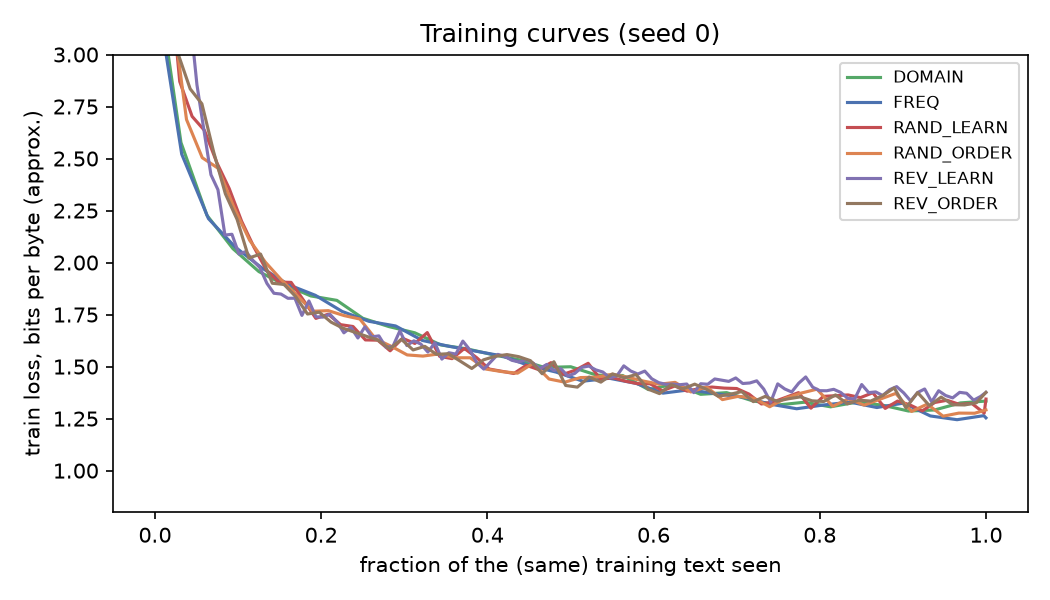
\includegraphics[width=0.7\linewidth]{figures/train_curves.png}
    \caption{Approximate per-byte training loss (seed 0) against the fraction of the shared training text seen. The curves overlap for most of training; the gaps open late, as \freq and \domain keep improving. Labels use underscores (\eg \texttt{REV\_LEARN} is \revlearn).}
    \label{fig:train_curves}
\end{figure}

\para{Compute.}
\Tabref{tab:compute} lists the training tokens, steps, and wall-clock time of each model.
Because all models see the same text, poor compressors take more steps.
Wall-clock times come from shared GPUs and are only a rough guide.

\begin{table}[h]
    \centering
    \caption{Pre-training compute for seed 0. Compute is relative to \freq (same model, so proportional to tokens). Poor compressors receive 1.7--3.8$\times$ more compute yet still reach worse \bpb.}
    \label{tab:compute}
    \small
    \begin{tabular}{@{}lcccc@{}}
        \toprule
        \textbf{Tokenizer} & \textbf{Train tokens} & \textbf{Steps} & \textbf{Minutes} & \textbf{Rel. compute} \\
        \midrule
        \freq                  & 51.0M  & 1,555 & 24.3 & 1.00$\times$ \\
        \domain                & 52.4M  & 1,600 & 18.4 & 1.03$\times$ \\
        \randlearn             & 110.0M & 3,358 & 33.2 & 2.16$\times$ \\
        \randlearn\textsc{-t1} & 112.7M & 3,438 & 56.8 & 2.21$\times$ \\
        \revlearn              & 194.6M & 5,939 & 32.4 & 3.82$\times$ \\
        \randorder             & 86.4M  & 2,637 & 28.6 & 1.70$\times$ \\
        \randorder\textsc{-t1} & 91.3M  & 2,787 & 45.4 & 1.79$\times$ \\
        \revorder              & 116.1M & 3,542 & 37.9 & 2.28$\times$ \\
        \bottomrule
    \end{tabular}
\end{table}

\para{Macro-F1.}
\Tabref{tab:f1} reports macro-F1, which tells the same story as accuracy.

\begin{table}[h]
    \centering
    \caption{Fine-tuned macro-F1 (\%, mean $\pm$ sd over 4 runs) and relative change against \freq. Best mean per task in \textbf{bold}. Mean test length in tokens is shown in parentheses, which reflects compression.}
    \label{tab:f1}
    \resizebox{\textwidth}{!}{%
    \begin{tabular}{@{}lccccccccc@{}}
        \toprule
        & \multicolumn{3}{c}{\sst} & \multicolumn{3}{c}{\agnews} & \multicolumn{3}{c}{\pubmedrct} \\
        \cmidrule(lr){2-4} \cmidrule(lr){5-7} \cmidrule(lr){8-10}
        \textbf{Tokenizer} & F1 & $\Delta$ & (len) & F1 & $\Delta$ & (len) & F1 & $\Delta$ & (len) \\
        \midrule
        \freq      & 80.2 {\scriptsize $\pm$ 0.4} & ---          & (30)  & \textbf{89.3} {\scriptsize $\pm$ 0.4} & ---          & (70)  & \textbf{75.4} {\scriptsize $\pm$ 0.5} & ---          & (37) \\
        \domain    & \textbf{81.4} {\scriptsize $\pm$ 0.4} & +1.57\%      & (31)  & 88.9 {\scriptsize $\pm$ 0.4} & $-$0.48\%    & (74)  & 75.4 {\scriptsize $\pm$ 0.2} & $-$0.08\%    & (34) \\
        \randlearn & 79.6 {\scriptsize $\pm$ 0.6} & $-$0.69\%    & (59)  & 88.8 {\scriptsize $\pm$ 0.4} & $-$0.58\%    & (131) & 75.1 {\scriptsize $\pm$ 0.6} & $-$0.49\%    & (83) \\
        \revlearn  & 80.7 {\scriptsize $\pm$ 0.7} & +0.66\%      & (104) & 88.7 {\scriptsize $\pm$ 0.4} & $-$0.72\%    & (213) & 74.8 {\scriptsize $\pm$ 0.2} & $-$0.91\%    & (140) \\
        \randorder & 79.7 {\scriptsize $\pm$ 0.7} & $-$0.54\%    & (47)  & 88.9 {\scriptsize $\pm$ 0.2} & $-$0.51\%    & (108) & 74.9 {\scriptsize $\pm$ 0.8} & $-$0.67\%    & (67) \\
        \revorder  & 80.0 {\scriptsize $\pm$ 0.9} & $-$0.23\%    & (63)  & 88.9 {\scriptsize $\pm$ 0.4} & $-$0.47\%    & (139) & 74.6 {\scriptsize $\pm$ 0.4} & $-$1.15\%    & (87) \\
        \bottomrule
    \end{tabular}}
\end{table}

\para{Implementation details.}
Our BPE trainer keeps a dictionary of pre-token counts and updates pair counts incrementally after each merge.
For the application-order tokenizers, we compute a dependency graph in which each merge points to the merges that use its output symbol, and we build a topological order of this graph by repeatedly choosing one merge whose inputs are already available: a uniformly random one for \randorder, and the latest-learned one for \revorder.
All experiments ran on shared NVIDIA RTX A6000 GPUs, using about 3\,GB of memory per job; each language model took 18--57 minutes.
We used PyTorch, HuggingFace \texttt{tokenizers}, NumPy, SciPy, pandas, and matplotlib.
